\documentclass[10pt]{article}
\usepackage[margin=20mm]{geometry}
\usepackage{enumitem}
\usepackage{hyperref}

\title{
Logbook of corrections 2020-07-03 
}
\author{Miguel Xochicale}
\date{ \today }

\begin{document}
\maketitle

\begin{abstract}
This logbook contains the suggested changes by Chris Baber 
presented in (\emph{.../corrections/2020-07-03/comments/README.md}),
fused text and further changes to the manuscript.
\end{abstract}


\tableofcontents

%%%%%%%%%%%%%%%%%%%%%%%%%%%%%%%%%%%%%%%%%%%%%%%%%%%%%%%%%%%%%%

\section{Comments}
\subsection{Text replacement}
\begin{enumerate}
\item 
"Perhaps you could replace your text with mine?  
\begin{verbatim}
Instead of replacing test, I will fuse text
\end{verbatim}
\textit{
SORTED: \\ 
Sun  4 Oct 01:11:27 BST 2020\\
}
\\
\end{enumerate}



\subsection{Experiment description}
\begin{enumerate}
\item 
"although still believe that there needs to be a bit more information in your description of the experiment, in terms of what participants had to do and in terms of the data collection"
\begin{verbatim}

Comestic changes changes to the experiment sections were made.
These include the subsections of particianpts, ethics, hhi activiites,
data collection from imus, raw data, data normalization smoothing, windowding

\end{verbatim}
\textit{
SORTED: \\ 
Sun 18 Oct 04:19:38 BST 2020
\\
}
\\
\end{enumerate}



\section{Introduction}

\subsection{ORIGINAL TEXT}
\begin{verbatim}
\section*{Introduction}
Human movement requires a complex system where not only multiple
joints and limbs are involved for a specific task in a determined environment
but also perception and action of movement that affects such 
physical performance \cite{davids2003}. 
In contrast, variability in humanoid movement is usually very small,
as a result of mechanical and dynamic capabilities \cite{gouaillier2009}. 
This means that, while humanoids 
solve the degrees of freedom problem through join design and algorithms,
humans tend to have more fluid and flexible approach. Consequently, 
one can see much variability in human movement performance of even the simplest task.
Studies of human motion reveal the possibility to 
estimate features from lower dimension signals to distinguish differences between 
styles of pedalling motion \cite{Quintana-Duque2012, Quintana-Duque2016}, 
gait identification \cite{sama2013, frank2010},
and detection of pathologies \cite{gomezgarcia2014}.
The lower dimension signals from biological systems are time series 
of $1-$dimension in $\mathbb{R}$ which commonly are 
noisy, nonlinear and non-stationary \cite{gomezgarcia2014}.
Hence, nonlinear dynamics can be used to 
objectively quantify variability of lower
dimension signals \cite{Quintana-Duque2012, Quintana-Duque2016, sama2013, 
frank2010, gomezgarcia2014, marwan2011, stergiou2011}.
For instance, Bradley et al. 2015 \cite{bradley2015} reviewed methods for
nonlinear time series analysis based on the estimation of the 
embedding parameters ($m$ embedding dimension and $\tau$ embedding delay) to 
reconstruct the state space,
where an $n$-dimensional reconstructed state space using $1-$dimensional 
time series,
can preserve the topological properties of an unknown $M$-dimensional 
state space \cite{takens1981}.
Similarly, Bradley et al. 2015 \cite{bradley2015} reviewed the use of 
Recurrence Plots (RPs), a graphical representation of a two-dimensional map 
which show black and white dots as recurrences in a given $n$-dimensional system, 
and Recurrence Quantification Analysis (RQA) metrics that compute statistics in RPs.
In general, RPs and RQA provide an intuitive meaning of the time series,
for instance, RQA is quantitatively and qualitatively independent of 
embedding dimension (also verified experimentally \cite{iwanski1998}).
However, the estimation of embedding parameters and the selection of the 
right parameters to perform RQA is still an open problem.
Bradley et al. 2015 \cite{bradley2015} pointed out that
there is no general technique that can be used to compute the embedding
parameters since time series are system-dependent which means that
computing the values for embedding parameters may only work for
one purpose (e.g., prediction) and may not work well for another purpose
(e.g., computing dynamical invariants).
Additionally, methods of nonlinear dynamics for 
computing embedding parameters e.g., autocorrelation, mutual information, 
and nearest neighbour require data which is well 
sampled and with little noise \cite{garland2016}
or require signals that are purely deterministic \cite{kantz2003}.
Thus, these methods of nonlinear analysis for computing the embedding 
parameters can break down
with real-world datasets which have generally different length, 
different values of accuracy and precision (rounding errors due to finite 
precision of the measurement apparatus which include frequency 
acquisition \cite{frank2010}),
and contaminated data with different sources of noise
\cite{garland2016}.
It is then surprising that even with the previous constraints with regard to 
the quality of data, and the problem with the estimation of embedding parameters,
the use of nonlinear dynamics have proven to be helpful to understand and 
to characterise dynamics of time series 
\cite{Quintana-Duque2012, Quintana-Duque2016, sama2013, frank2010,
gomezgarcia2014, gomezgarcia2014, marwan2011, stergiou2011, bradley2015}.

%Another point to consider with time series analysis using nonlinear dynamics
%is the appropriate use of different post-processing techniques such as 
%interpolation, filtering or normalisation.
%With that in mind, it can be said that there is little research and 
%understanding on the effects for post-processing techniques
%in the interpretation of reconstructed state spaces, RPs and RQA.

For this work, we are interested in exploring and investigating  
the effects of different features of time series 
(e.g. levels of smoothness, window data length,
structures of time series based on types of movements, 
types of sensors, participants and velocities) to estimate 
embedded parameters for uniform time-delay embedding, 
recurrence plots and recurrence quantification analysis.
Hence, we conducted an experiment with twenty right-handed 
healthy participants in the context of human-humanoid imitation 
activities where participants were asked to 
imitate simple arm movements performed by a humanoid robot.
The primary aim of this work is to explore the following questions:
\begin{itemize}
\item What are the effects on three nonlinear methods 
	(reconstructed state space with uniform time-delay embedding, 
	Recurrence Plots, and Recurrence Quantification Analysis), 
	for different embedding parameters, different recurrence thresholds 
	and different characteristics of time series 
	(structure of the signal, window length and smoothness of the signal)?, and 
\item What are the strengths and weaknesses of Recurrence
	Quantification Analysis for the previous conditions
	of nonlinear analysis methods?

\end{verbatim}


\subsection{SUGGESTED TEXT}
\begin{verbatim}
The complexity of human movement arises from the balancing of consistency 
and variability in solving the Degrees of Freedom problem (Bernstein, xx). 
Each joint can be moved in more than one plane, leading to many possible 
combinations which need to be reduced into order to perform a control action (Newell, xx). 
However, too much reduction can result in highly consistent movement which lacks 
sufficient variability to allow adaptation to situational demands. 
Consequently, one can see much variability in human movement even the 
simplest of movements.  Variability can be beneficial in supporting adaptability 
and can reflect experience and expertise of the performance, e.g., in cycling.  
Uncontrolled variability, due to disease, disfunction or inexperience, 
can be detrimental to performance and plays a role in detection of pathologies. 
While the analysis of movement of variability is becoming increasingly 
popular as a diagnostic tool, there remain challenges in terms of defining 
the most appropriate methods and parameters to apply. In part, 
these challenges stem from the fact that the identification movement 
variability requires analysis of signals which are time-series of 1-dimension 
in R which are noisy, nonlinear and non-stationary.  
Further problems arise from assigning a plausible locus of control to 
the movements, e.g., in order to determine whether variability is the 
result of deliberative control by the performer or whether it arises 
from exogenous or endogenous disturbances.  For this paper, our focus 
is on the analysis of signals; specifically, in terms of objectively 
quantifying variability of lower dimension signals using time-series analysis.

Methods for time-series analysis generally involve the estimation 
of embedding parameters (m embedding dimension and T embedding delay) 
which are used to reconstruct the n-dimensional state space of 
the 1-dimension time-series.  Key to the selection of these 
parameters is the need to ensure that the topological properties 
of the (unknown) M-dimensional state space.   A popular approach 
to the construction of these state spaces involves the use of 
Recurrence Plots (RPs) which provide a graphical two-dimensional 
map (using black and white dots) to indicate recurring patterns 
in the n-dimensional system.  While RPs provide a human 
interpretable picture of the system, these require further 
analysis to allow the properties of that system to be quantified, 
and so Recurrence Quantification Analysis (RQA) can be applied.  
However, the estimation of the embedding parameters for 
RQA remains an open problem (Bradley et al., 2015).

There is no agreed method for estimating embedding parameters 
(for RQA or for other nonlinear analysis methods) because time-series 
are system-dependent, i.e., these rely on the initial conditions, 
and on the configuration and behaviour of the system.  
This means that, unless one holds all of the influencing 
variables constant, embedding parameters computed for one 
instance may not apply to another instance.   
One could apply methods, such as autocorrelation, mutual information, 
nearest neighbour (and we will apply these in this paper), 
but these methods assume that the data are well sampled, with 
little noise and (usually) that the signals are purely deterministic.  
As such, these methods can break-down in the face of real-world datasets 
which could have different length, different degrees of precision, or 
different levels of contamination from exogenous and endogenous 
sources of ‘noise’.  What is, perhaps, surprising is that 
even subject to these problems, the methods are useful and 
nonlinear dynamics approaches continue to tell us much about 
human movement.

For this paper, we explore the role of RP and RQA in the 
analysis of simple human movement.  We compare horizontal and 
vertical arm movements performed by neurotypical participants 
who are copying these movements being made by a humanoid robot.  
This provides an initial point of comparison 
(between human movement, which we assume to have a degree of variability, 
and the robot, which we assume to have a degree of consistency).   
Additionally, our interest lies in the estimation of embedding parameters 
in light of different features of the data, e.g., levels of smoothing, 
window length, structure of time-series based on movement, 
types of sensors, individual differences between participants and 
the movements that they perform. Specifically, we ask what are 
the effects of different embedding parameters, recurrence thresholds 
and characteristics of time-series on nonlinear analysis 
methods (i.e., reconstructed state space with 
uniform time-delay embedding, Recurrence Plots and 
Recurrence Quantification Analysis)?

\end{verbatim}





\subsection{FUSED TEXT}
\begin{verbatim}

\section*{Introduction}
The complexity of human movement arises from the process of mastering 
redundant (bio)mechanical degrees of freedom (DOF) to successfully 
accomplish any given motor task (Bernstein, 1967).
Such DOF are independent coordinates to uniquely 
describe the configuartions of the system which provides flexibiity 
and stability to adapt to a change enviroment conditions but 
that leads many possible combinations (Newell and Vaillancourt, 2001).
Hence, human movement complexity can be seen as a balance 
between the required DOF "to generate a stable (persistent) 
and flexible (variable) behavioural output in response to 
changing intentions and dynamic environmental
conditions" \cite{davids2003}. 
Consequently, one can see much variability in human movement even the 
simplest of movements.  
While the analysis of movement of variability is becoming increasingly 
popular as a diagnostic tool or skill performance evaluation, 
there remain challenges in terms of defining 
the most appropriate methods and parameters to apply. 
In part, 
these challenges stem from the fact that the identification movement 
variability requires analysis of signals which are time-series of 
of $1-$dimension in $\mathbb{R}$ which are 
noisy, nonlinear and non-stationary \cite{gomezgarcia2014}.
Further problems arise from assigning a plausible locus of control to 
the movements, e.g., in order to determine whether variability is the 
result of deliberative control by the performer or whether it arises 
from exogenous or endogenous disturbances.  For this paper, our focus 
is on the analysis of signals; specifically, in terms of objectively 
quantifying variability of lower dimension signals using time-series analysis.

Methods for nonlinear time series analysis generally involve the estimation of the 
embedding parameters ($m$ embedding dimension and $\tau$ embedding delay) to 
reconstruct the state space,
where an $n$-dimensional is reconstructed state space using $1-$dimensional 
time series \cite{Quintana-Duque2012, Quintana-Duque2016, sama2013, 
frank2010, gomezgarcia2014, marwan2011, stergiou2011}.
Key to the selection of these parameters is the need to preserve 
topological properties of an unknown $M$-dimensional state space \cite{takens1981}.
An common approach to the construction of these state spaces 
involves Recurrence Plots (RPs), a graphical representation of black and white dots, 
which shows recurrent patterns of a $n$-dimensional system.
While RPs provide a human
interpretable picture of the system, these require further
analysis to allow the properties of that system to be quantified,
and so Recurrence Quantification Analysis (RQA) can be applied.
However, the estimation of the embedding parameters for
RQA remains an open problem (Bradley et al. 2015 \cite{bradley2015})
There is no agreed method to estimate embedding parameters
for RQA and other nonlinear methods \cite{bradley2015} 
because time series are system-dependent, i.e., these rely
on the initial conditions, and on the configuration and behaviour of the system.  
This means that, unless one holds all of the influencing 
variables constant, embedding parameters computed for one 
instance may not apply to another instance.   

One could apply methods, such as autocorrelation, mutual information, 
nearest neighbour (and we will apply these in this paper), 
but these methods assume that the data are well sampled, with 
little noise and (usually) that the signals are purely deterministic \cite{garland2016, kantz2003}.
That said, these methods can break-down in the face of real-world datasets 
which could have 
different length, 
different values of accuracy and precision (rounding errors due to finite 
precision of the measurement apparatus which include frequency 
acquisition \cite{frank2010}), or 
different levels of contamination from exogenous and endogenous 
sources of ‘noise’ \cite{garland2016}.  What is, perhaps, surprising is that 
even subject to these problems, the methods are useful and 
nonlinear dynamics approaches continue to tell us much about 
human movement \cite{Quintana-Duque2012, Quintana-Duque2016, sama2013, frank2010,
gomezgarcia2014, marwan2011, stergiou2011, bradley2015}.

For this paper, we explore the role of RPs and RQA in the 
analysis of simple human movement. 
We compare horizontal and 
vertical arm movements performed by neurotypical participants 
who are copying these movements being made by a humanoid robot.  
This provides an initial point of comparison 
(between human movement, which we assume to have a degree of variability, 
and the robot, which we assume to have a degree of consistency).   
Additionally, our interest lies in the estimation of embedding parameters 
in light of different features of the data, e.g., levels of smoothing, 
window length, structure of time-series based on movement, 
types of sensors, individual differences between participants and 
the movements that they perform. 
Specifically, we ask what are 
the effects of different embedding parameters, recurrence thresholds 
and characteristics of time-series on nonlinear analysis 
methods (i.e., reconstructed state space with 
uniform time-delay embedding, RPs and RQA)?

\end{verbatim}


\textit{
SORTED: \\ 
Tue 11 Aug 18:37:21 BST 2020 \\
Sun 18 Oct 04:27:51 BST 2020
\\
}



\section{Results}
\subsection{ORIGINAL TEXT}
\begin{verbatim}

\section*{Results}

\subsection*{Reconstructed State Spaces}
One of the challenges of the implementation of 
uniform time-delay embedding to reconstruct the state spaces is the 
selection of embedding parameters because each time series is unique in 
terms of its structure (e.g. modulation of amplitude, frequency and phase) 
\cite{ frank2010, sama2013, bradley2015}.
With that in mind, the problem for this work is not to compute individual 
embedding parameters for each of the time series but to deal with a 
selection of two parameters that can represent all the time series. 
Our solution for such problem, as explained in below sections, 
was to compute a sample mean over all 
values in each of the conditions of the time series 
%of Figs~\ref{fig:ts}
for minimum dimension values and 
%Figs~\ref{fig:caoami} 
for minimum delay values.
%, resulting in an average minimum embedding parameters 
%of ($\overline{m_0}=6$, $\overline{\tau_0}=8$).

\subsubsection*{Minimum embedding parameters}
Minimum embedding parameters were firstly computed 
with the methods of False Nearest Neighbour and Average Mutual Information.
%for Uniform Time-Delay Embedding (UTDE),
%Reconstructed State Space (RSS), 
%Recurrence Plots (RPs) and 
%Recurrence Quantification Analysis (RQAs).
Figures \ref{fig:cao_ami}(A) show box plots for the minimum embedding values 
for sensors HS01 and RS01. Minimum embedding vaues for HS01 presents more 
variations than RS01 as interquartile range for HS01 is near to 1 (with the exceptions of HF sg0, VN sg0, and VF sg1)
whereas interquartile range for RS01 is near to 0.1 (with the exception of two axis HF sg0 and VF sg1).
Additionally, Figures \ref{fig:cao_ami}(A) show
a decrease of mean values (rhombus) in the box plots
as smoothness of time series increase (see sg0, sg1, sg2).
Figures \ref{fig:cao_ami}(B) show box plots for the first minimum values of AMI values.
It can be seen that values for HS01 tend to be more spread as the smoothness 
of the time series is increasing 
(see the increase of both mean (rhombus) and interquartile range).
However, AMI values for RS01 do not show such increase in relation with
the increase of smoothness except for HF and VF
(Figs \ref{fig:cao_ami}(B)).

We also computed a sample mean for an overall minimum embedding parameters that 
represent all participants, activities, sensors and levels of smoothness.
The sample mean for the minimum values of $E_{1}(m)$ from Figs \ref{fig:cao_ami}(A) 
is $\overline{m}_0=6$ 
and the sample mean for minimum values of AMIs from Figs~\ref{fig:cao_ami}(B)
is $\overline{\tau}_0=8$.
%Hence, we use the average minimum embedding parameters 
%($\overline{m_0}=6$, $\overline{\tau_0}=8$) to compute 
%Reconstructed State Spaces (RSSs), Recurrence Plots (RPs) and
%Recurrence Quantification Analysis (RQA) metrics for human-humanoid activities.
%---------------------------------(FIGURE)-------------------------------------
\begin{figure}[ht]
\centering
\includegraphics[width=1.0\textwidth]{figures/caoami/pdf/fig2}
	\caption{
	{\bf Box plots of minimum embedding parameters.} 
	Box plots of (A) minimum embedding dimensions 
	and (B) first minimum AMI values for 
	Horizontal Normal (HN), Horizontal Faster (HF),
	Vertical Normal (VN) and Vertical Faster (VF)
	with sensors attached to participants (HS01) and
	sensor attached to robot (RS01).
	Minimum embedding parameters are for twenty participants 
	($p01$ to $p20$) with three smoothed signals 
	(sg0: sg0zmuvGyroZ, sg1: sg1zmuvGyroZ and sg2: sg2zmuvGyroZ)
	and window length of 10-sec (500 samples).
	Code and data to reproduce the figure is available in \cite{srep2020}.
        }
    \label{fig:cao_ami}
\end{figure}
%%---------------------------------(FIGURE)------------------------------------

\subsubsection*{Uniform Time-Delay Embedding}
Uniform time-delay embedding were computed with the overall 
embedding parameters ($\overline{m_0}=6$, $\overline{\tau_0}=8$) and 
the first three axis of the rotated data of the PCA are shown 
for the reconstructed state spaces of horizontal arm movements
(Figs~\ref{fig:rss_aHw10}) and vertical arm movements 
(Figs~\ref{fig:rss_aVw10}).
%%---------------------------------(FIGURE)-------------------------------------
\begin{figure}[ht]
\centering
\includegraphics[width=1.0\textwidth]{figures/rss/pdf/fig3}
\caption{
	{\bf RSSs for horizontal arm movements.}
	Reconstructed state spaces for time series for p01 of Figure \ref{fig:ts}.
	Reconstructed state spaces were computed with 
	embedding parameters 
	$\overline{m}_0=6$, $\overline{\tau}_0=8$.
	Code and data to reproduce the figure is available in \cite{srep2020}.
        }
    \label{fig:rss_aHw10}
\end{figure}
%%---------------------------------(FIGURE)------------------------------------
%%---------------------------------(FIGURE)-------------------------------------
\begin{figure}[ht]
\centering
\includegraphics[width=1.0\textwidth]{figures/rss/pdf/fig4}
    \caption{
	{\bf RSSs for vertical arm movements.}
	Reconstructed state spaces for time series for p01 of Figure \ref{fig:ts}.
	Reconstructed state spaces were computed with 
	embedding parameters
	$\overline{m}_0=6$, $\overline{\tau}_0=8$.
	Code and data to reproduce the figure is available in \cite{srep2020}.
        }
    \label{fig:rss_aVw10}
\end{figure}
%%---------------------------------(FIGURE)------------------------------------

One can observe by eye the differences in each of the
trajectories of the reconstructed state spaces 
(Figs~\ref{fig:rss_aHw10} and \ref{fig:rss_aVw10}), 
however an objective quantification is required.
That being said, we tried to quantify those differences 
using euclidean distances between the origin 
to each of the points in their trajectories, 
which results did not capture the dynamics of 
the trajectories specially 
for those that looked very messy.
Such ambiguities lead us to consider the use of 
Recurrence Plots and Recurrence Quantification Analysis 
to objectively quantify dynamics the capture activities 
using time series.


\subsection*{Recurrences Plots}
Recurrence Plots (RP) were computed for horizontal arm movements (Fig~\ref{fig:rp_aH}) and 
vertical arm movements (Fig~\ref{fig:rp_aV}) 
using the average embedding parameters 
($\overline{m}_0=6$, $\overline{\tau}_0=8$) 
and an recurrence threshold of $\epsilon=1$.
%%---------------------------------(FIGURE)-------------------------------------
\begin{figure}[ht]
\centering
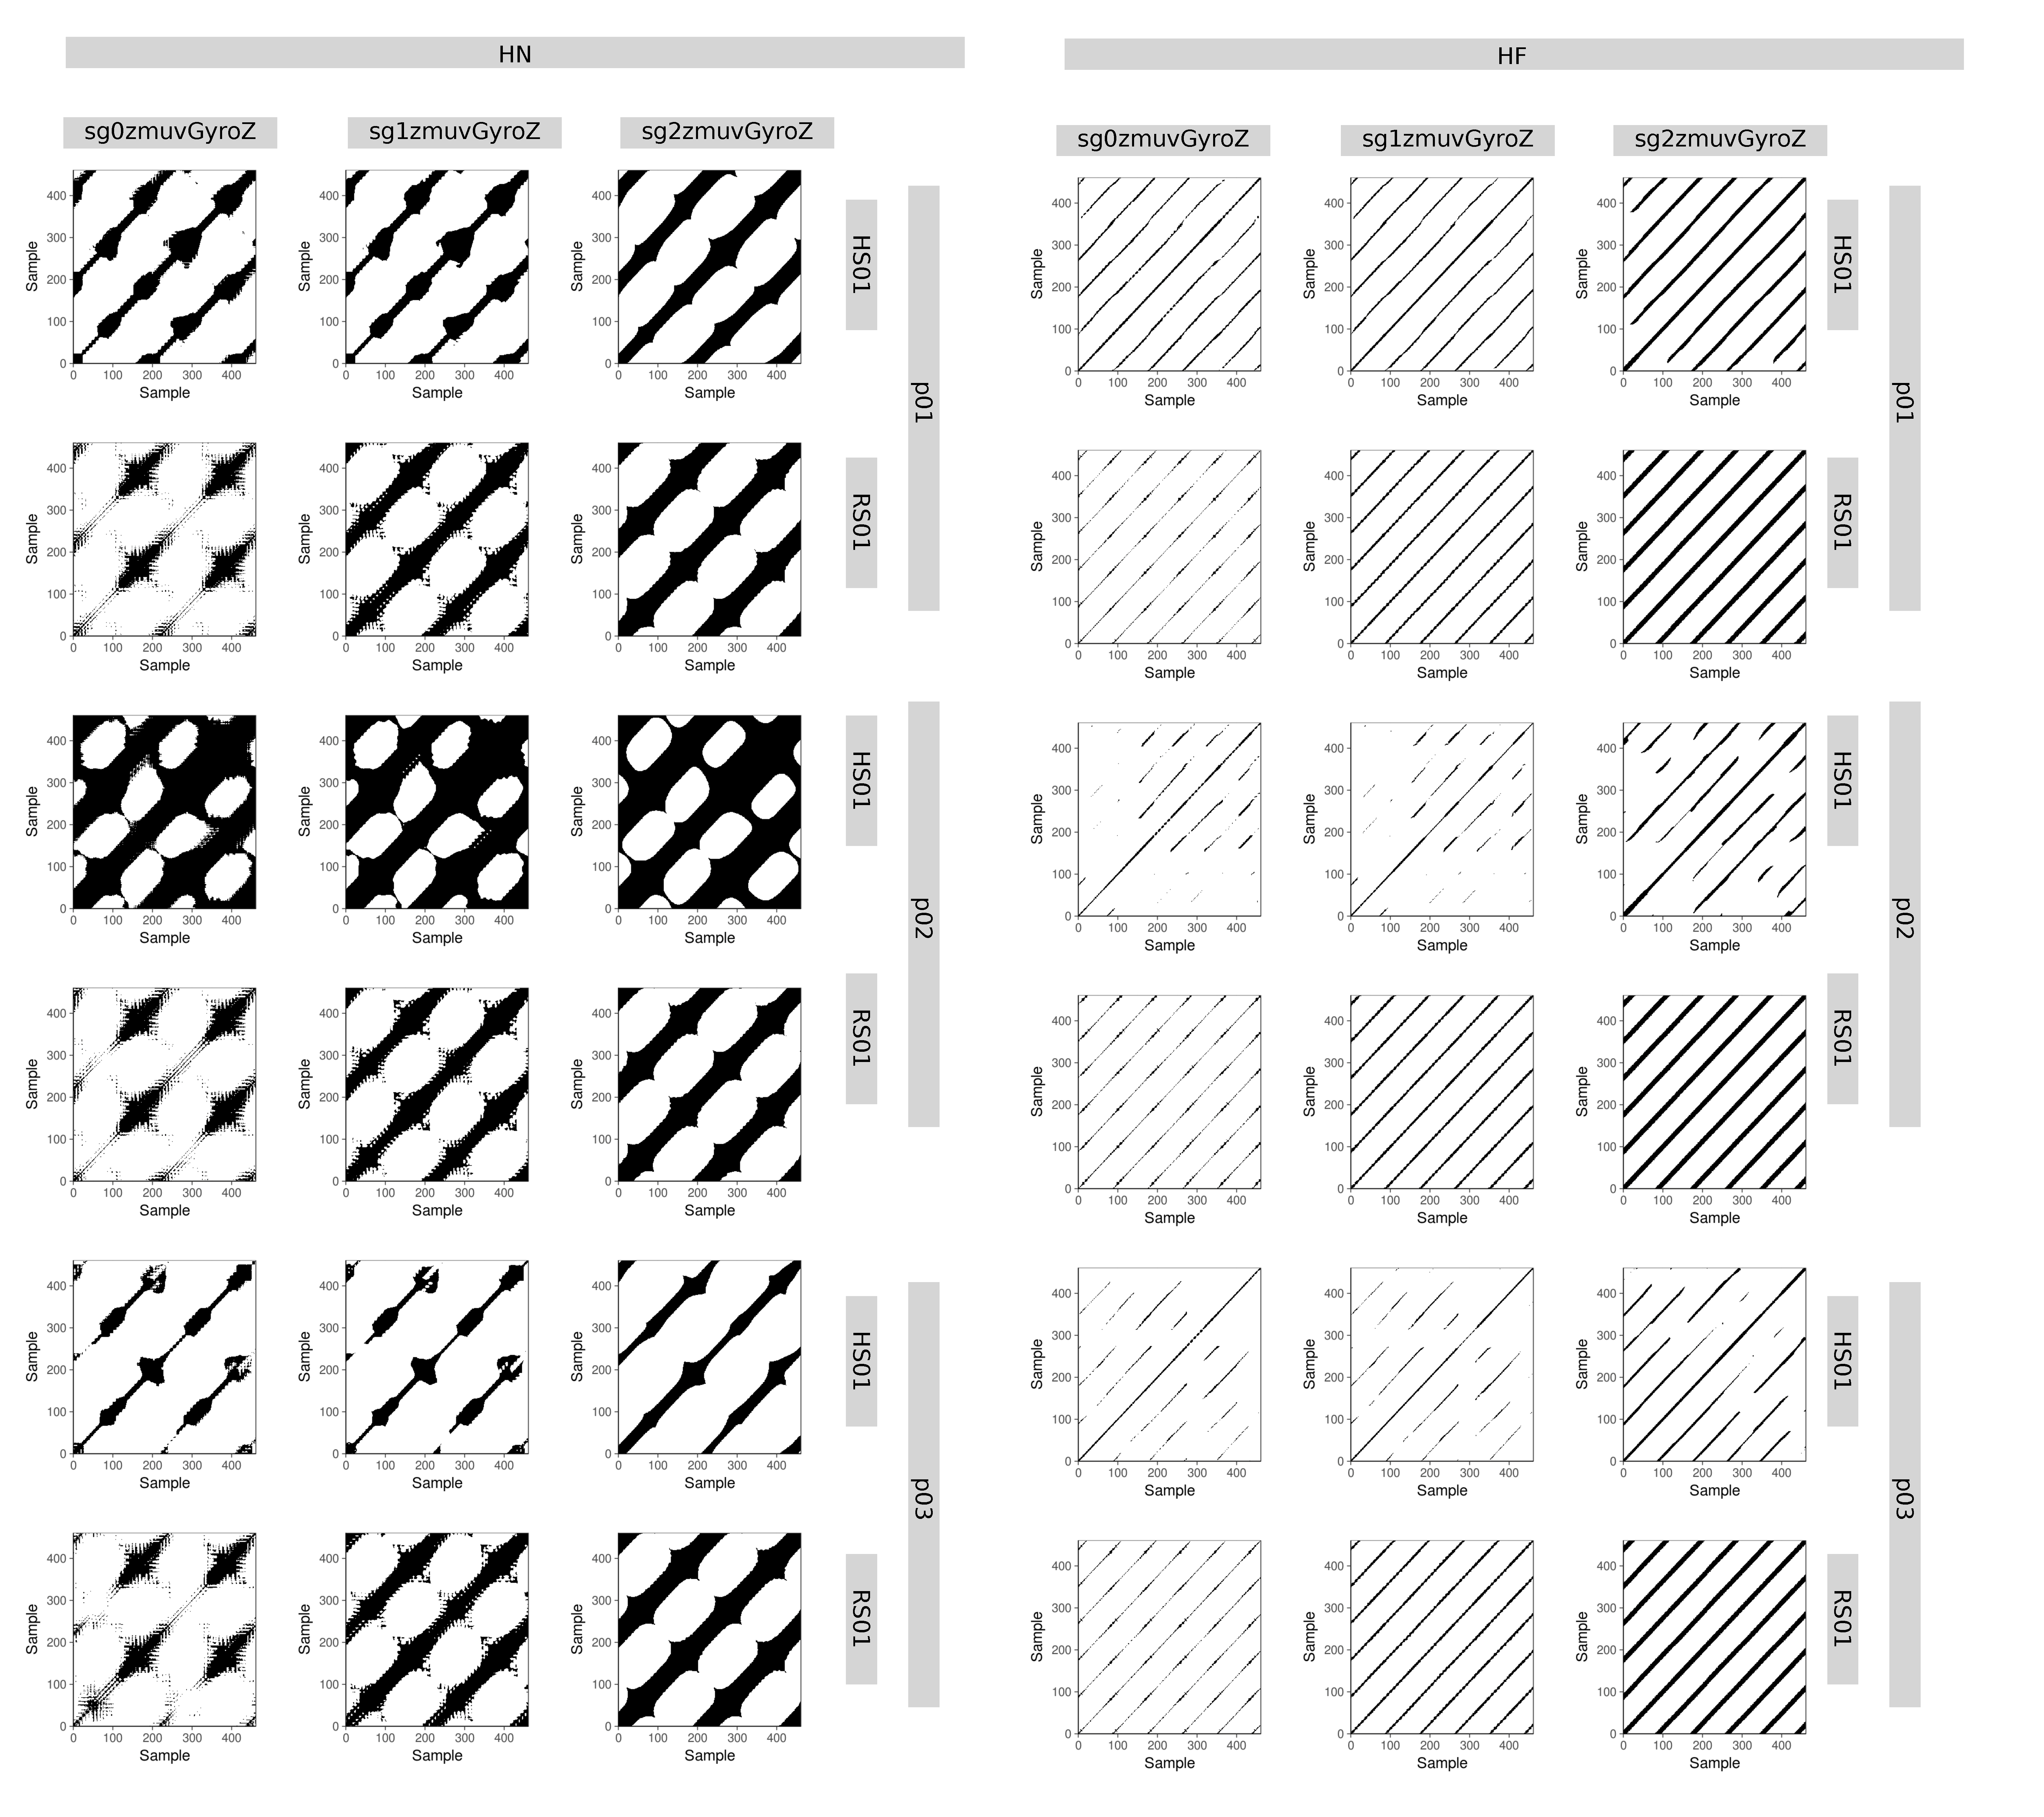
\includegraphics[width=1.0\textwidth]{figures/rps/pdf/rp_aH}
\caption{
	{\bf RPs for horizontal arm movements.}	
	Recurrence plots were computed with 
	embedding parameters 
	$\overline{m}_0=6$, $\overline{\tau}_0=8$, and $\epsilon=1$.
	Code and data to reproduce the figure is available in \cite{srep2020}.
        }
    \label{fig:rp_aH}
\end{figure}
%%---------------------------------(FIGURE)------------------------------------
%%---------------------------------(FIGURE)-------------------------------------
\begin{figure}[ht]
\centering
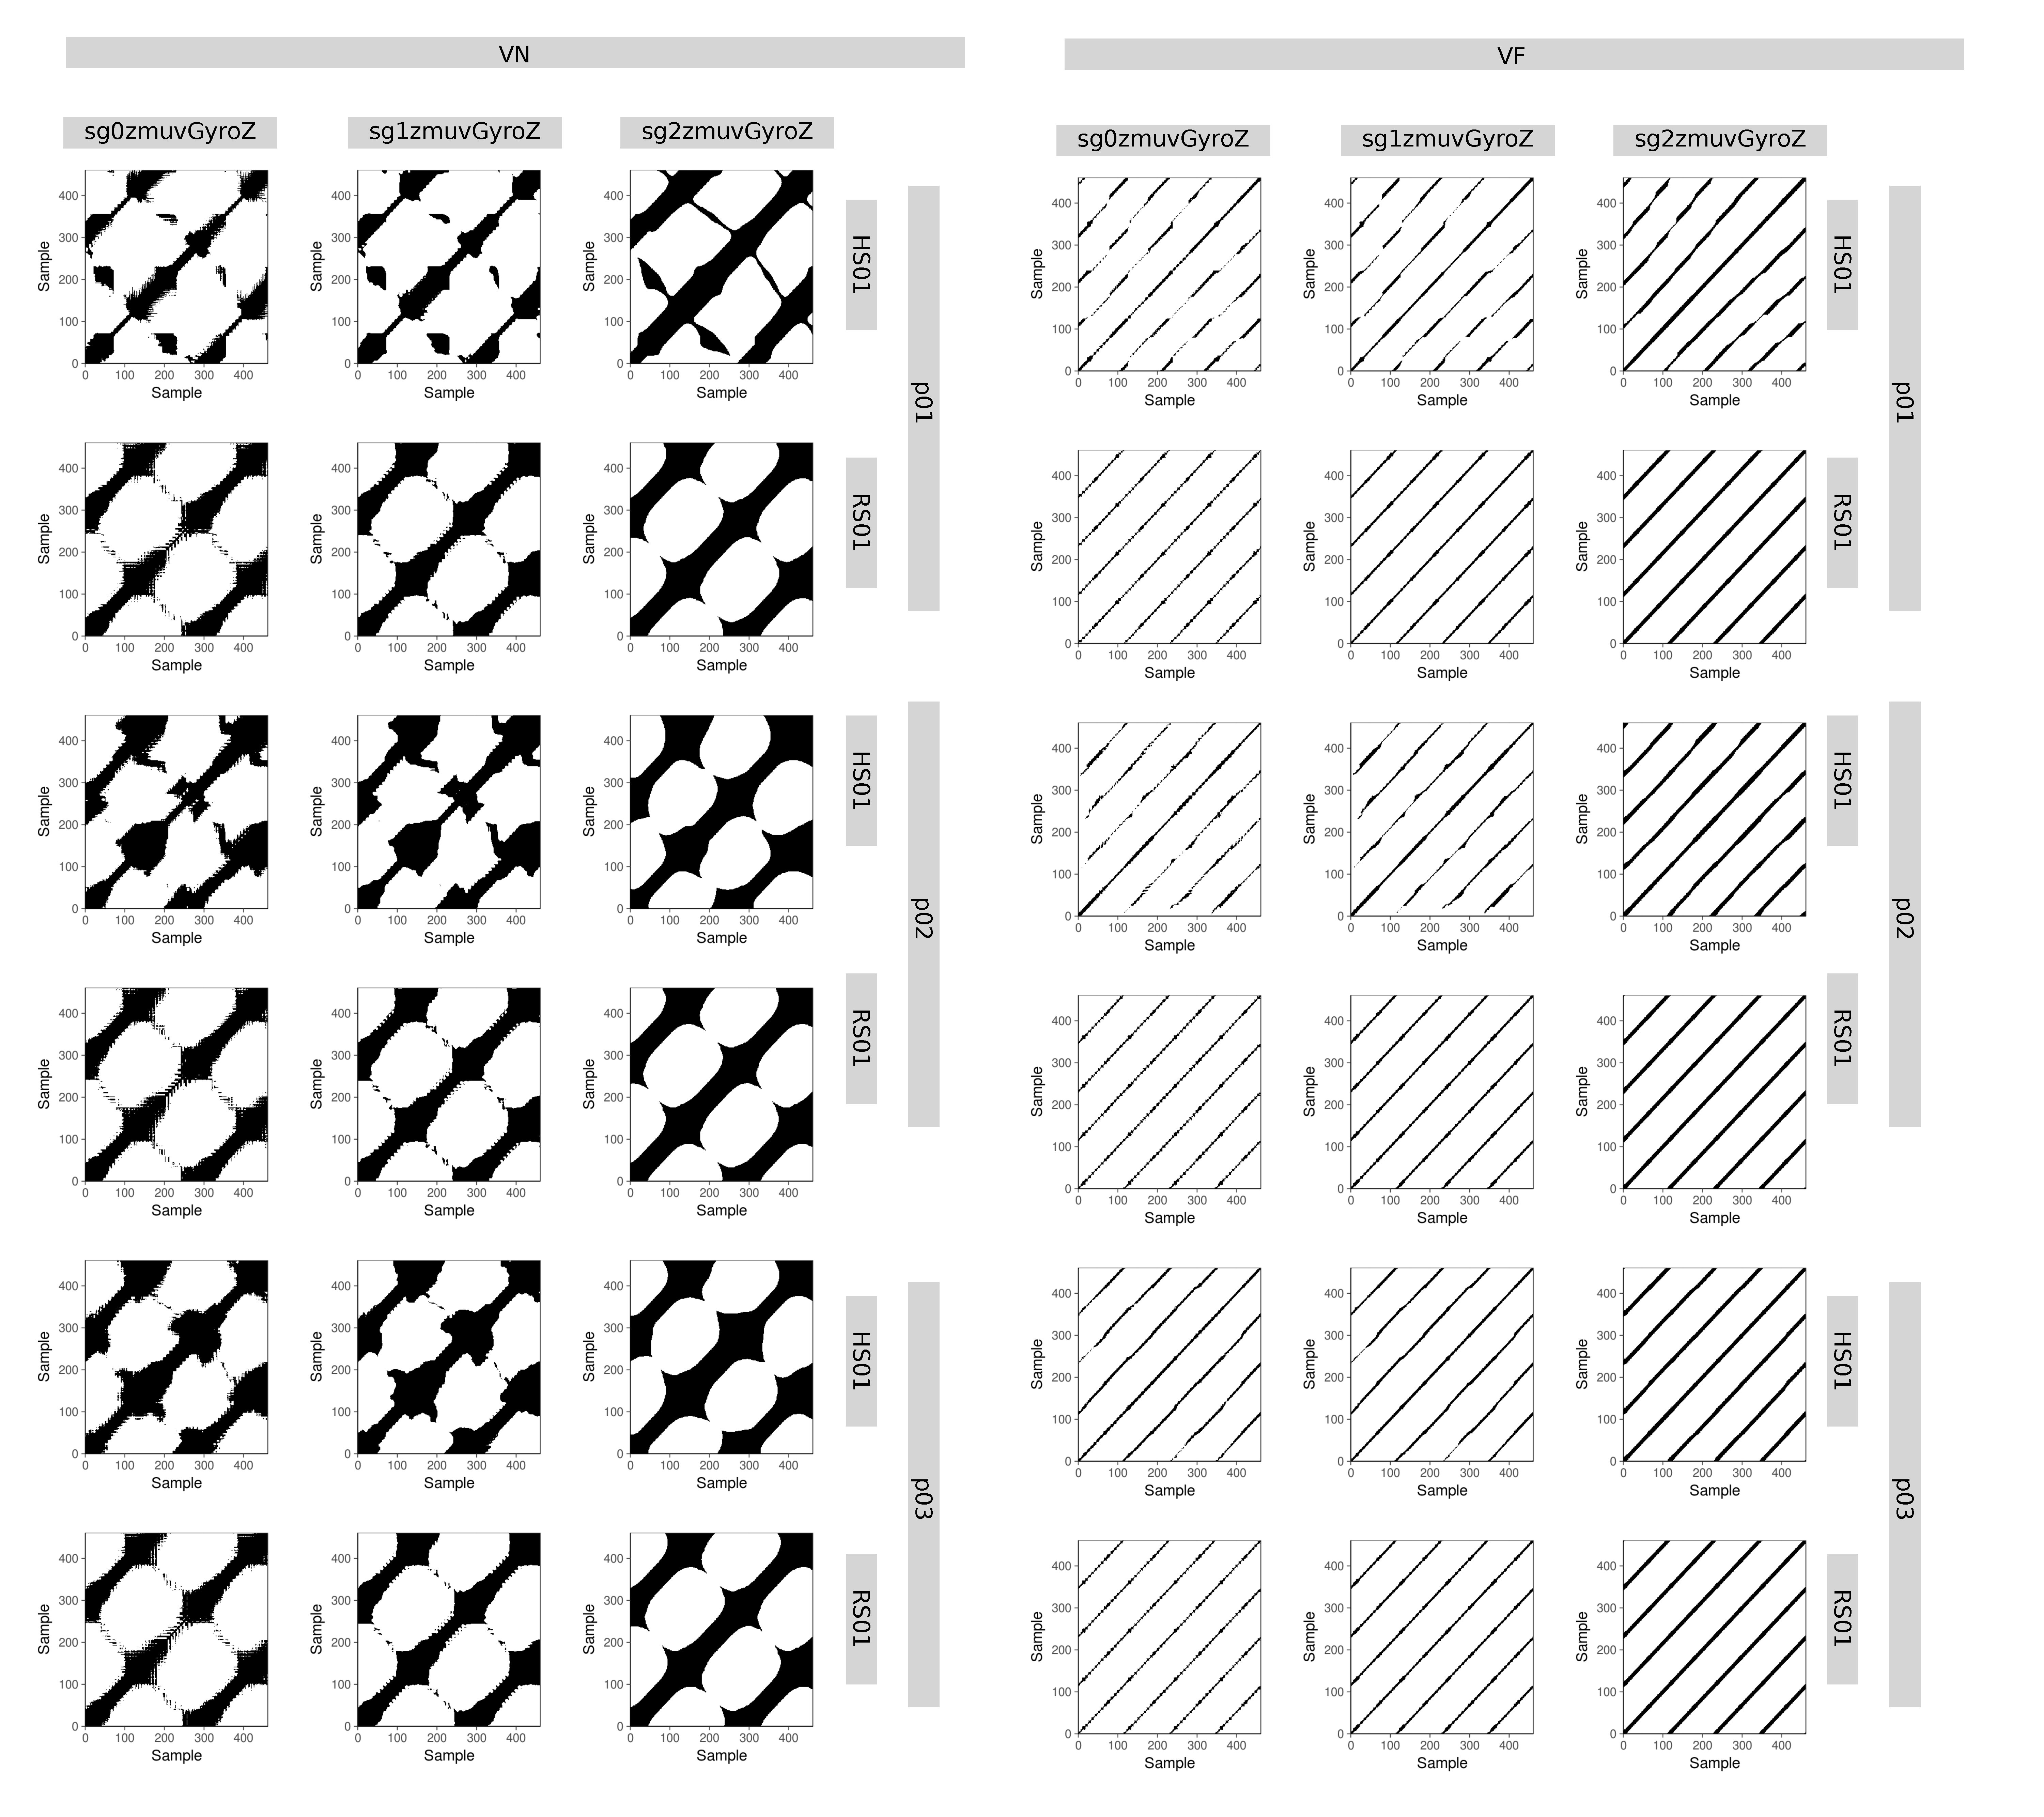
\includegraphics[width=1.0\textwidth]{figures/rps/pdf/rp_aV}
\caption{
	{\bf RPs for vertical arm movements.}	
	Recurrence plots were computed with 
	$\overline{m}_0=6$, $\overline{\tau}_0=8$, and $\epsilon=1$.
	Code and data to reproduce the figure is available in \cite{srep2020}.
        }
    \label{fig:rp_aV}
\end{figure}
%%---------------------------------(FIGURE)------------------------------------


\subsection*{Recurrence Quantification Analysis} \label{ch6:rqas}
Four Recurrence Quantification Analysis (RQA) metrics (REC, DET, RATIO and ENTR) 
were also computed with $\overline{m}_0=6$, $\overline{\tau}_0=8$, and $\epsilon=1$. 
 
\subsubsection*{REC values}
Figs~\ref{fig:RQABP}(A) show box plots of REC values 
that represent the \% of black dots in RPs.
It can be noted that REC values are more spread 
for HN and VN movements (higher interquartile range) than 
for HF and VF movements (lower interquartile range) for HS01 sensor. 
In contrast, REC values for RS01 sensor present little variation 
(interquartile range of 0.01).
Regarding the increase of smoothness for time series 
(sg0, sg1 and sg2), REC values present little 
variation as the smoothness is increasing for time series from HS01 
(changes of mean values (rhombus)) whereas REC values are 
more affected with the smoothness for data from RS01 
(see the incremental changes of mean values (rhombus)).
%See Figs~\ref{fig:rec_aH} and \ref{fig:rec_aV} in appendix \ref{appendix:e:ep} 
%for more details about individual REC values for each participant.


\subsubsection*{DET values}
Figs \ref{fig:RQABP}(B) illustrate DET values 
that represent the predictability and organisation of RPs.
Generally, it can be noted little change of DET values 
(interquartile range is around 0.1) 
for type of movement, type of sensor 
but the increase of DET values as the smoothness of 
the signal increase 
(see the incremental changes of mean values (rhombus)).
However, the interquartile range for faster movements
(HF and VF) with no smoothing (sg0) is lower than the other
levels of smoothness (sg1 and sg2).
%See Figs~\ref{fig:det_aH} and \ref{fig:det_aV} in appendix \ref{appendix:e:ep} 
%for more details about individual DET values for each participant.

\subsubsection*{RATIO values}
Figs \ref{fig:RQABP}(C) illustrate RATIO values that represent the 
dynamic transitions in RPs. 
Generally, it can be seen that RATIO values for HS01 sensor vary less 
for HN movements (interquartile range around 2)
than HF movements (interquartile range around 5).
For faster movements (HF and VF), it can be noted a decrease of 
the mean values the smoothness of the time series 
is increasing (rhombus). However, for normal movements (HN and VN), 
the decrease of mean values is less evident than 
faster movements (rhombus).
%See Figs~\ref{fig:ratio_aH} and \ref{fig:ratio_aV} in appendix 
%\ref{appendix:e:ep} 
%for more details about individual RATIO values for each participant.


\subsubsection*{ENTR values}
Figs \ref{fig:RQABP}(D) show ENTR values that represent 
Shannon entropy values in RPs. 
Generally, 
ENTR values for HS01 sensor show a higher variation  
(interquartile range around 0.5)
than ENTR values for RS01 sensor 
(interquartile range 0.1).
It can also be noted the increase of mean values 
for ENTR values as the smoothness of time series 
increase (rhombus) for type of movement, 
type of sensor and level of smoothness.  
%See Figs~\ref{fig:entr_aH} and \ref{fig:entr_aV} in appendix
%\ref{appendix:e:ep}
%for more details about individual ENTR values for each participant.


%%---------------------------------(FIGURE)-------------------------------------
\begin{figure}
\centering
\includegraphics[width=1.0\textwidth]{figures/rqa/output/rqa-bp}
    \caption
	[Box plots for RQA values]{
	{\bf Box plots for RQA metrics.}
	RQA metrics for (A) REC, (B) DET, (C) RATIO, and (D) ENTR of 
	20 participants performing HN, HF, VN and VF movements
	with sensors HS01, RS01 and three smoothed-normalised  
	time series (sg0, sg1 and sg2).
	RQA values were computed with 
	$\overline{m}_0=6$, $\overline{\tau}_0=8$, and $\epsilon=1$. 
	Code and data to reproduce the figure is available in \cite{srep2020}.
        }
    \label{fig:RQABP}
\end{figure}
%%---------------------------------(FIGURE)------------------------------------


%\subsection*{RQA metrics with fixed parameters}
%Considering that RQA metrics were computed with fixed embedding parameters 
%($m=6$ and $\tau=8$) and recurrence thresholds ($\epsilon=1$), we found 
%the following. REC values, which represents the \% of black points in the RPs, 
%were more affected with and increase in normal speed movements (HN and VN) 
%than faster movements (HF and VF) for the sensor attached to the participants 
%(HS01). Such decrease of REC values from normal speed to faster speed 
%movements is also presented in data from sensor attached to the robot (RS01), 
%and little can be said with regard to the dynamics of the time series coming 
%from RS01 (Fig \ref{fig:RQABP}A).
%Similarly, DET values, representing predictability and 
%organisation in the RPs, present little variation in the any of the time 
%series where little can be said (Fig \ref{fig:RQABP}B).
%In contrast, RATIO values, which represent 
%dynamic transitions, were more variable for faster movements (HF and VF) 
%than normal speed movements (HN and VN) with sensors attached to the 
%participants (HS01). For data coming from sensors attached to the robot 
%(RS01), RATIO values from horizontal movements (HN, HF) appear to vary 
%more than values coming from vertical movmentes (VN, VF) 
%(Fig \ref{fig:RQABP}C).
%With that, it can be said that RATIO values can represent a bit better
%than REC or DET metrics for the variability of imitation activities in 
%each of the conditions for time series.
%Similarly, ENTR values for HN were higher than values for HF
%and ENTR values varied more for sensor attached to participants 
%than ENTR values for sensors of the robot. It is evidently that 
%the higher the entropy the more complex the dynamics are, 
%however, ENTR values for HN appear a bit higher than HF values, 
%for which we believe this happens because of the structure the time series
%which appear more complex for HN than  HF movements which presented a 
%more consistence repetition (Fig \ref{fig:RQABP}D).


\subsection*{3D RQA ENTR}
To show how that the selection of recurrence threshold affects RQA
values, 
we computed ENTR values of RQA metrics for different embedding parameters
$ \{ m \in \mathbb{R} | 1 \le m \le 10  \} $,
$  \{ \tau \in \mathbb{R} | 1 \le \tau \le 10  \} $ incrementing by one,
with the consideration of three recurrence thresholds $\epsilon=1, 2, 3$ 
and three levels of smoothness (sg0, sg1, sg2). 
For instance, 
Figures \ref{fig:RQA-IND} show the increase of recurrence threshold is 
associated to the increase of ENTR values in any of the levels 
of smoothness (see values of the ENTR bar).
Similarly, it can be noted that the increase of level of 
smoothness (sg0, sg1 and sg2) is associated with the increase 
of ENTR values of the 3D surface plots.
%%---------------------------------(FIGURE)-------------------------------------
\begin{figure}
\centering
\includegraphics[width=1.0\textwidth]{figures/rqa/output/rqa-epsilons}
    \caption
	[3D surface plots of RQA ENTR values]{
	{\bf 
	3D surface plots of RQA ENTR values for different recurrence threshold and smoothness levels.}
	RQA ENTR values are
	for embedding parameters
	$ \{ m \in \mathbb{R} | 0 \le m \le 10  \} $,
	$ \{ \tau \in \mathbb{R} | 0 \le \tau \le 10  \} $
	incrementing by one and three recurrence thresholds $\epsilon=1, 2, 3$.
	RQA ENTR values were computed with data from $p03$, sensor HS01, with 
	a window size of 10-secs (500 samples).
	Code and data to reproduce the figure is available in \cite{srep2020}.
        }
    \label{fig:RQA-IND}
\end{figure}
%%---------------------------------(FIGURE)------------------------------------
Figures~\ref{fig:3dRQAENTR_sensoractivities} show 3D surface plots of 
ENTR values for different sensors and different activities.
Figs~\ref{fig:3dRQAENTR_sensoractivities} show that RQA ENTR (lateral bars) 
decrease from normal (HN, VN) to faster (HF, VF) velocities from both 
human sensor (HS01) to robot sensor (RS01).
Also, it can be noted that RQA ENTR values decrease from human sensor (HS01) 
to robot sensor (RS01).
%%---------------------------------(FIGURE)-------------------------------------
\begin{figure}[ht]
\centering
\includegraphics[width=1.0\textwidth]{figures/rqa/output/rqa-sensors-activities}
    \caption{
	{\bf 3D surface plots of RQA ENTR values for different sensors and activities.}
	RQA ENTR values are for embedding parameters
	$ \{ m \in \mathbb{R} | 0 \le m \le 10  \}$,
	$ \{ \tau \in \mathbb{R} | 0 \le \tau \le 10  \}$
	with $\epsilon = 1 $ considering four activities 
	Horizontal Normal (HN), Horizontal Faster(HF), Vertical Normal(VN), and 
	Vertical Faster (VF) and sensors Human Sensor 01 (HS01) and 
	Robot Sensor (RS01).
	RQA ENTR values were computed from data of $p03$, sg0 and 
	window size of 10-secs (500 samples).
	Code and data to reproduce the figure is available in \cite{srep2020}.
       }
\label{fig:3dRQAENTR_sensoractivities}
\end{figure}
%%---------------------------------(FIGURE)-------------------------------------
Figures~\ref{fig:3dRQAENTR_participantsactivities} show the similarity of 3D surface plots in 
relationship with three participants (p01, p02 and p03)
performing four activities (HN, HF, VN, and VF) and two sensors (HS01, RS01).
Figures~\ref{fig:3dRQAENTR_participantsactivities}(A) 
present subtle differences for each of the participants (see RQA ENTR bar). 
Figures~\ref{fig:3dRQAENTR_participantsactivities}(B) show 
less change of RQA ENTR values for each participant as the data is 
from a sensor attached to the robot. 
Also, from data of sensors attached to the robot, it can be noted 
that changes are more notable for faster movements than normal movements. 
%%---------------------------------(FIGURE)-------------------------------------
\begin{figure}[ht]
\centering
\includegraphics[width=0.9\textwidth]{figures/rqa/output/rqa-participants}
    \caption{
	{\bf 3D surface plots of RQA ENTR values for different participants, activities and sensors.}
	RQA ENTR values are for participants (p01, p02, and p03) 
	in the categories of 
	(A) Human Sensor 01 (HS01) and 
	(B) Robot Sensor 01 (RS01)
	considering embedding parameters
	$ \{ m \in \mathbb{R} | 0 \le m \le 10  \}$,
	$ \{ \tau \in \mathbb{R} | 0 \le \tau \le 10  \}$
	with $\epsilon = 1$ and four activities 
	Horizontal Normal (HN), Horizontal Faster(HF), Vertical Normal(VN), and 
	Vertical Faster (VF).
	RQA ENTR values were computed from data of sg0 and window size of 10-secs (500 samples).
	Code and data to reproduce the figure is available in \cite{srep2020}.
       }
\label{fig:3dRQAENTR_participantsactivities}
\end{figure}
%%---------------------------------(FIGURE)-------------------------------------
Figures \ref{fig:3dRQAENTR_windowsactivities} show the effect of the increase 
of window length of the time series (w100 (2-sec), w250 (5-sec), w500 (10-sec) and w750 (15-sec))
on the 3D surface plots. 
It can be noted that the increase of number of samples improves the quality 
of the surface plots where 100 samples poorly capture the dynamics of each activity.
However as the window length increases from 250, 500 to 750 samples, 
3D surface plots show a similar representation of RQA ENTR values 
(being the surface plot with 750 samples the best test case).
%%---------------------------------(FIGURE)-------------------------------------
\begin{figure}[ht]
\centering
\includegraphics[width=1.0\textwidth]{figures/rqa/output/rqa-windows}
    \caption{
	{\bf 3D surface plots of RQA ENTR values for different windows lengths and activities.}
	RQA ENTR values are for embedding parameters
	$ \{ m \in \mathbb{R} | 0 \le m \le 10  \}$,
	$ \{ \tau \in \mathbb{R} | 0 \le \tau \le 10  \}$, 
	with $\epsilon = 1 $ considering four 
	windows lengths (e.g., w100 (100 samples), w250 (250 samples),
	w500 (500 samples) and w750 (750 samples)) and
	four activities 
	Horizontal Normal (HN), Horizontal Faster(HF), Vertical Normal(VN), and 
	Vertical Faster (VF).
	RQA ENTR values were computed from data of $p01$ and sg0.
	Code and data to reproduce the figure is available in \cite{srep2020}.
       }
\label{fig:3dRQAENTR_windowsactivities}
\end{figure}
%%---------------------------------(FIGURE)-------------------------------------

To summarise this section of results, it can be said that computing
embedding parameters for individual structure of time-series 
data is already a solved problem \cite{frank2010, sama2013, bradley2015}. 
However, it has been shown the challenge of finding embedding parameters 
for nonlinear dynamic tools that represent a set of different time-series data.
That said, we proposed the use of sample mean of the set of embedding parameters
for RSSs, RP and RQA to then noticed that the selection of recurrence 
threshold, $\epsilon$, is also an open problem.
For which, this work proposed the variation of recurrence thresholds 
and embedding parameters to show the relationships of these to different datasets 
(participants, activities, windows lengths and sensors).




\end{verbatim}





\subsection{SUGGESTED TEXT}
\begin{verbatim}

Reconstructed State Spaces
As noted in the Introduction, a challenge in the implantation of uniform time-delay embedding 
arises from the selection of embedding parameters because of the uniqueness of each time series 
in terms of its structure (e.g., modulation of amplitude, frequency, phase etc.). 
With that in mind, the options are to either calculate embedding parameters for each unique 
instance (which can make comparison challenging) or to find parameters which can apply to all 
instances in the study.  We recognise that the latter approach is not without its problems, 
but our approach is to compute sample mean over all values in each of the conditions of the 
time series for minimum dimension and minimum delay values.

Minimum embedding parameters
Minimum embedding parameters were initially computed using False Nearest Neighbour (FNN) 
and Average Mutual Information (AMI).   We used FNN to calculate a value for m 
and AMI to calculate a value for X? Comment: You should provide a sentence here 
to justify the use these different methods for m and X? 
To illustrate this, figure (A) show box plots for minimum embedding values for sensors 
on the wrist of the human (HS01) and the robot (RS01).   
As we had assumed, minimum embedding values for HS01 show greater variation than 
those for RS01 (as indicated by differences in interquartile ranges).  
Additionally, figure (A) show a decrease in mean values (rhombus) in the box plots 
as smoothness of the time-series increases (see sg0, sg1, sg2).  
Figure (B) show box plots for Average Mutual Information (AMI).  
One can see that, in contrast to RS01, minimum values for HS01 tend to spread 
as the smoothness of the time-series increases.
The sample mean for minimum value of embedding parameter, m derived from 
FNN  (figures A) is 6 and  Tfrom AMI (figures B) is 8.

Uniform Time-delay embedding
Using the minimum embedding parameters (defined above), 
the first three axis of the rotated Principal Components Analysis (PCA) 
are shown for the reconstructed state spaces of horizontal (figures  ) 
and vertical (figures ) arm movements.   While visual inspection of these figures 
suggests differences in the trajectories of the reconstructed state spaces, 
we require an objective quantification to determine the extent of the differences.  
One approach could be use Euclidean distances from the origin for points in these 
trajectories, but this proved inconclusive and was not able to capture 
the dynamics of the trajectories. Consequently, we applied RP and RQA.

Recurrence Plots
Using the minimum embedding parameters and a recurrence threshold of 1 
Comment: you should explain why you chose 1 here Recurrence Plots (RP) were 
computed for horizontal (figures ) and vertical (figures ) arm movements.

Recurrence Quantification Analysis
Four Recurrence Quantification Analysis metrics (percentage recurrence, REC, 
representing the percentage of black dots in RP; percentage determinism, DET, 
representing the predictability of the RP; ratio of DET / REC, RATIO; 
Shannon entropy, ENTR) were computed using the same parameters as for RP.

REC values
Figure (A) presents box plots of REC which show that REC values, 
for HS01, are more spread for Slow (i.e., 5 seconds per movement) movements 
in Horizontal (HS) or Vertical (VS) than for Fast (i.e., 2 seconds per movement).  
This suggests greater variation between participants for the Slow movements.  
For RS01, there is little variation between Slow and Fast movement.  
In terms of smoothness, there seems little effect of HS01 but RS01 values 
do show affects of smoothness.

DET values
Figure (b) presents DET values and shows little difference for type of movement or performer.  
However, DET values are affected by changes in smoothness of the signal, 
particularly for Fast movement.

RATIO values
Figure (C) presents the ratio of DET / REC.  These values, for the human performer, 
vary less for HN than for HF movement.  
Additionally, smoothness leads to a decrease in mean values for Fast movements.

ENTR values
Figure (d) shows ENTR values are higher for the human performer than the robot, 
and vary with the smoothness of the time-series.

3D RQA ENTR
As ENTR appeared to be have higher sensitivity than the other measures, 
we explored the impact of different embedding parameters /{m.../}, /{.../} 
incrementing by 1 each run, with recurrence thresholds e = 1,2,3 and levels of 
smoothness (sg0, sg1, sg2).  
Figure ( ) shows that increasing recurrence 
threshold leads to an increase in ENTR regardless of level of smoothness.  
Increasing level of smoothness will also increase ENTR (figure () ).  
In terms of movement or performer, RQA ENTR decrease from Slow (HS, VS) to Fast (HF, VF) 
for both human and robot.   In terms of individual differences, for human participants, 
figure ( ) compares p01, p02 and p03 (for illustrative purposes) – 
both between each other and in comparison with the more consistent performance of the robot.  
In terms of window length (w100 (2s), w250 (5s), w500(10s), w750 (15s)), figure ( ) 
shows that improvement in capture with number of samples, although this has less 
of an effect on RQA ENTR.

\end{verbatim}


\subsection{FUSED TEXT}
\begin{verbatim}

%*******************************************************************************
%*******************************************************************************
\section*{Results}

\subsection*{Reconstructed State Spaces}
As noted in the Introduction, a challenge in the implementation of uniform time-delay embedding 
arises from the selection of embedding parameters because of the uniqueness of each time series 
in terms of its structure (e.g., modulation of amplitude, frequency, phase etc.). 
With that in mind, the options are to either calculate embedding parameters for each unique 
instance (which can make comparison challenging) or to find parameters which can apply to all 
instances in the study.
We recognise that the latter approach is not without its problems, 
but our approach is to compute sample mean over all values in each of the conditions of the 
time series for minimum dimension and minimum delay values.

\subsubsection*{Minimum embedding parameters}
Minimum embedding parameters were initially computed using False Nearest Neighbour (FNN) 
and Average Mutual Information (AMI).   We used FNN to calculate a value for $m$
to unfold the attractors and AMI to calculate a value for $\tau$ and maxime the 
information in the unfolded attractor.
To illustrate this, figure \ref{fig:cao_ami} (A) show box plots for minimum embedding 
values for sensors on the wrist of the human (HS01) and the robot (RS01).   
As we had assumed, minimum embedding values for HS01 show greater variation than 
those for RS01 (as indicated by differences in interquartile ranges).  
Additionally, figure \ref{fig:cao_ami} (A) show a decrease in mean values (rhombus) in the box plots 
as smoothness of the time-series increases (see sg0, sg1, sg2).  
Figure \ref{fig:cao_ami} (B) show box plots for Average Mutual Information (AMI).  
One can see that, in contrast to RS01, minimum values for HS01 tend to spread 
as the smoothness of the time-series increases.
The sample mean for minimum value of embedding parameter, 
$m$ derived from FNN  (figures \ref{fig:cao_ami} A) is $\overline{m}_0=6$ 
and $\tau$ from AMI (figures \ref{fig:cao_ami} B) is $\overline{\tau}_0=8$.

%---------------------------------(FIGURE)-------------------------------------
\begin{figure}[ht]
\centering
\includegraphics[width=1.0\textwidth]{figures/caoami/pdf/fig2}
	\caption{
	{\bf Box plots of minimum embedding parameters.} 
	Box plots of (A) minimum embedding dimensions 
	and (B) first minimum AMI values for 
	Horizontal Normal (HN), Horizontal Faster (HF),
	Vertical Normal (VN) and Vertical Faster (VF)
	with sensors attached to participants (HS01) and
	sensor attached to robot (RS01).
	Minimum embedding parameters are for twenty participants 
	($p01$ to $p20$) with three smoothed signals 
	(sg0: sg0zmuvGyroZ, sg1: sg1zmuvGyroZ and sg2: sg2zmuvGyroZ)
	and window length of 10-sec (500 samples).
	Code and data to reproduce the figure is available in \cite{srep2020}.
        }
    \label{fig:cao_ami}
\end{figure}
%%---------------------------------(FIGURE)------------------------------------

\subsubsection*{Uniform Time-Delay Embedding}
Using the overall embedding parameters ($\overline{m_0}=6$, $\overline{\tau_0}=8$), 
the first three axis of the rotated Principal Components Analysis (PCA) 
are shown for the reconstructed state spaces of horizontal (figures~\ref{fig:rss_aHw10}) 
and vertical (figures~\ref{fig:rss_aVw10}) arm movements. 
While visual inspection of these figures 
suggests differences in the trajectories of the reconstructed state spaces, 
we require an objective quantification to determine the extent of the differences.  
One approach could be use Euclidean distances from the origin for points in these 
trajectories, but this proved inconclusive and was not able to capture 
the dynamics of the trajectories. Consequently, we applied 
Recurrence Plots and Recurrence Quantification Analysis.

\subsection*{Recurrences Plots}
Using the average embedding parameters 
($\overline{m}_0=6$, $\overline{\tau}_0=8$) 
and an recurrence threshold of $\epsilon=1$.
As our interest is for dynamical transitions, 
there is little importance on the selection of $\epsilon$ which in this case
is 1. 
Recurrence Plots (RP) were computed for horizontal (figures~\ref{fig:rp_aH}) and 
vertical (figures~\ref{fig:rp_aV}) arm movements.


\subsection*{Recurrence Quantification Analysis} \label{ch6:rqas}
Four Recurrence Quantification Analysis metrics (
percentage recurrence, REC, representing the percentage of black dots in RP; 
percentage determinism, DET, representing the predictability of the RP; 
ratio of DET / REC, RATIO; Shannon entropy, ENTR) 
were computed using the same parameters as for RP.
%\subsubsection*{REC values}
Figure~\ref{fig:RQABP}(A) presents box plots of REC values, 
for HS01, are more spread for Slow (i.e., 5 seconds per movement) movements 
in Horizontal (HS) or Vertical (VS) than for Fast (i.e., 2 seconds per movement).  
This suggests greater variation between participants for the Slow movements.  
For RS01, there is little variation between Slow and Fast movement
(interquartile range of 0.01). 
In terms of smoothness, there seems little effect of HS01 but RS01 values 
do show affects of smoothness (see the incremental changes of mean values (rhombus)).
%\subsubsection*{DET values}
Figure \ref{fig:RQABP}(B) presents DET values and shows 
little difference for type of movement or performer.  
However, DET values are affected by changes in smoothness of the signal, 
particularly for Fast movement.
%\subsubsection*{RATIO values}
Figure \ref{fig:RQABP}(C) presents the ratio of DET / REC. 
These values, for the human performer, vary less for HN than for HF movement.  
Additionally, smoothness leads to a decrease in mean values for Fast movements.
%\subsubsection*{ENTR values}
Figure \ref{fig:RQABP}(D) shows ENTR values are higher for the human 
performer than the robot, and vary with the smoothness of the time-series.

\subsection*{3D RQA ENTR}
As ENTR appeared to be have higher sensitivity than the other measures, 
we explored the impact of different embedding parameters 
$ \{ m \in \mathbb{R} | 1 \le m \le 10  \} $,
$  \{ \tau \in \mathbb{R} | 1 \le \tau \le 10  \} $ 
incrementing by 1 each run, with recurrence thresholds $\epsilon=1, 2, 3$ 
and levels of smoothness (sg0, sg1, sg2).  
Figure \ref{fig:RQA-IND} shows that increasing recurrence 
threshold leads to an increase in ENTR regardless of level of smoothness.  
Similarly, increasing level of smoothness will also increase ENTR (figure \ref{fig:RQA-IND}).
In terms of movement or performer, RQA ENTR decrease from Slow (HS, VS) to Fast (HF, VF) 
for both human (HS01) and (RS01) (Figures~\ref{fig:3dRQAENTR_sensoractivities}).
In terms of individual differences, for human participants, 
figure \ref{fig:3dRQAENTR_participantsactivities} compares p01, p02 and p03 (for illustrative purposes) --
both between each other and in comparison with the more consistent performance of the robot.  
In terms of window length (w100 (2s), w250 (5s), w500(10s), w750 (15s)), 
figure \ref{fig:3dRQAENTR_windowsactivities} shows that improvement in 
capture with number of samples, although this has less of an effect on RQA ENTR.




\end{verbatim}



\textit{
SORTED: \\ 
Tue  1 Sep 23:43:03 BST 2020\\
Sat  3 Oct 14:54:05 BST 2020\\
Sat  3 Oct 23:55:12 BST 2020 \\
}
\\


\section{Discussion}

\subsection{ORIGINAL TEXT}
\begin{verbatim}

\section*{Discussion}
Time series from different sources  
(e.g., participants, movements, axis type) as well as
different characteristics (e.g., sample rate, window length or levels of smoothness) 
result in different embedding parameters and therefore different 
values for recurrence plots and recurrence quantification analysis metrics.
That said, while embedding parameters for individual
time series were successfully computed, the quantification 
of variability with regard to the shape of the trajectories in 
reconstructed state spaces require more investigation
as our initial, approach based on euclidean distances on the trajectories, 
failed to quantify trajectories which were not well unfolded. 
To then found out that Recurrence Plots along with 
Recurrence Quantification Analysis (RQA) metrics (e.g., REC, DET, RATIO and ENTR) 
and its variation of embedding parameters and recurrence thresholds 
helped to quantify the variability of different sources of time series.
However, further investigation is required to be done in order to 
have better intuition and meaningful interpretation of nonlinear 
analysis such as to find a right 
balance among (i) the level of smoothness of the signal, 
(ii) the selection of recurrence thresholds and (iii) 
the range of embedding parameters. 

\end{verbatim}

\subsection{SUGGESTED TEXT}
\begin{verbatim}

While there are many approaches to estimating embedding parameters for nonlinear analysis, 
these can be influenced by the structure of the time-series data.   
We show that, for RSS, RP and RQA, the estimation of embedding parameters can be performed 
using a sample mean which, together with recurrence threshold, can be shown to be 
influenced by activity, performer, window length and smoothness of time-series.  
It is known that time-series from different sources and with different characteristics 
require different embedding parameters, and this can produce different RPs.  
We have shown how RQA metrics can help to quantify movement variability.

\end{verbatim}


\subsection{FUSED TEXT}
\begin{verbatim}

\section*{Discussion}
While there are many approaches to estimating embedding parameters for nonlinear analysis, 
these can be influenced by the structure of the time-series data.   
We show that, for RSS, RP and RQA, the estimation of embedding parameters can be performed 
using a sample mean which, together with recurrence threshold, can be shown to be 
influenced by activity, performer, window length and smoothness of time-series.  
It is known that time-series from different sources and with different characteristics 
require different embedding parameters, and this can produce different RSS, RPs and RQAs. 
Although this work helps to understand the open problem of 
finding right balance among (i) the level of smoothness of the signal, 
(ii) the selection of recurrence thresholds and (iii) 
the range of embedding parameters, 
we have shown how RQA metrics can help to quantify movement variability.




\end{verbatim}



\textit{
SORTED: \\ 
Sun  4 Oct 00:52:04 BST 2020\\
}
\\





\section{Conclusions}


\subsection{ORIGINAL TEXT}
\begin{verbatim}


\section*{Conclusions}
This work allows to conclude that the choice of 
nonlinear analysis tool (e.g., RSSs, RPs, RQA metrics) will depend 
on what one would like to quantify on the time-series 
data (e.g., predicability, organisation, dynamics transitions, 
or complexity and determinism).
Then, time-series data characteristics 
(e.g., window size length, level of smoothness) plays an important role
as well on the results that nonlinear analysis tool can provide.
Similarly, the results of the nonlinear analysis tools
are associated with the structure of the time-series data 
(e.g. frequency, amplitude), the position of the sensor 
and activity performed by either a robot or human being
(as degrees of freedom from the humanoid are far less than
human movement). 
That said, it has been shown that the use of different 
characteristics of the time-series data 
(e.g., sensor, activity, level of smoothness and participants)
has help us to visualise and to quantify 
with nonlinear tools the variation of 
movements of, in this work, human-humanoid activities.
However, some limitation of nonlinear tools are related 
to the computation of different parameters 
(e.g., recurrence thresholds, embedding parameters)
that reflect the dynamics of individual characteristics 
of activity type, window length and structure of the time series.
Specifically, the example of DET values which appear 
to be constants across sensors, activities and levels of smoothness, 
whereas REC and RATIO, as function of REC, values 
show variation for certain sensors and movements. 
To then found out that RQA ENTR values with different recurrence 
thresholds were appropriate to quantify 
the different changes and variations of the characteristics of 
time-series data.
Therefore, we can conclude that this work provides a good starting 
point and reference to the use of Shannon Entropy to quantify 
human-humanoid imitation activities 
that can then lead to interesting results on the quantification 
of movement variability of participants with different ages, 
state of health and anthropomorphic features.


\end{verbatim}








\subsection{SUGGESTED TEXT}
\begin{verbatim}
In this paper we show how the selection of nonlinear analysis metric 
(i.e., RSS, RP, RQA metrics) depends on what question one wishes to 
address with time-series data (e.g., predictability, organisation, dynamics, complexity).  
Time-series data characteristics (e.g., window length, smoothness), 
time-series structure (e.g., frequency, amplitude) and 
data source (e.g., sensor placement, performance, movement) all influence the results. 
That said, it has been shown that the use of different characteristics of the data and 
their collection can help us visualise and quantify variability of movement using 
methods of nonlinear analysis.   
There remain limitations of nonlinear methods in 
relation to the estimation of parameters (e.g., recurrence threshold, embedding parameters) 
which reflect the dynamics of specific movement and performers, window length 
and structure of the time-series. 
We note that RQA DET seems to show low sensitivity 
to these differences, whereas REC and RATIO (primarily as a result of REC) show 
variation across performers and movements.   
RQA ENTR, with different recurrence thresholds, 
can quantify variation in the time-series data and offers the most appropriate means 
for analysing variability in movement to allow us to analyse individual differences 
between human performers.  

This metric could be applied to analyse human participants 
who might vary in age, state of health, anthropometric features and capability to perform movement."


\end{verbatim}


\subsection{FUSED TEXT}
\begin{verbatim}


\section*{Conclusions}
In this paper we show how the selection of nonlinear analysis tool  
(i.e., RSS, RP, RQA metrics) depends on what question one wishes to 
address with time-series data (e.g., predictability, organisation, dynamics, complexity).  
Time-series data characteristics (e.g., window length, smoothness), 
time-series structure (e.g., frequency, amplitude) and 
data source (e.g., sensor placement, performance, movement) all influence 
the results that nonlinear analysis methods can provide.
That said, it has been shown that the use of different characteristics of the data and 
their collection can help us visualise and quantify variability of movement using 
methods of nonlinear analysis.   
There remain limitations of nonlinear methods in 
relation to the estimation of parameters (e.g., recurrence threshold, embedding parameters) 
which reflect the dynamics of specific movement and performers, window length 
and structure of the time-series. 
We note that RQA DET seems to show low sensitivity 
to these differences, whereas REC and RATIO (primarily as a result of REC) show 
variation across performers and movements.   
RQA ENTR, with different recurrence thresholds, 
can quantify variation in the time-series data and offers the most appropriate means 
for analysing variability in movement to allow us to analyse individual differences 
between human performers.  
To then found out that RQA ENTR values with different recurrence 
thresholds were appropriate to quantify 
the different changes and variations of the characteristics of 
time-series data.
Therefore, the use of Shannon Entropy could be applied 
to analyse human participants who might vary in age, 
state of health, anthropometric features and capability to perform movement.


\end{verbatim}

\textit{
SORTED: \\ 
Sun  4 Oct 01:10:47 BST 2020 \\
}
\\


\section{Abstract}

\subsection{ORIGINAL TEXT}
\begin{verbatim}



\begin{abstract}
Human movement variability occurs in motor performance 
across multiple repetitions of a task and such behaviour is an
inherent feature within and between each persons' movement. Quantifying
movement variability is still an open problem, particularly 
when methods in time domain, frequency domain or nonlinear dynamics 
can break down due to the real-world time-series datasets. 
For this work, we therefore investigate nonlinear dynamics methods 
such as reconstructed state space (RSSs), uniform time-delay embedding, 
recurrence plots (RPs) and recurrence quantification analysis metrics (RQAs)
with real-world time-series data.
Particularly, we are interested in the weaknesses and robustness 
of nonlinear dynamics tools with the use of raw and post-processed 
data of wearable inertial sensors. 
That said, twenty right-handed healthy participants 
imitated simple vertical and horizontal arm movements in normal 
and faster velocity from an humanoid robot in order to have 
four window lengths and three levels of smoothed time-series data,
to then found visual differences in the patterns with RSSs and RPs
and particulatly the computed differences with RQA metrics
that help us to quantify activities, types of sensors, windows lenghts 
and level of smoothness. 
Specifically, we can conclude that RQA ENTR, Shannon Entropy, 
can lead to interesting results on the quantification of 
movement variablity for participants of different ages, 
state of health and anthropomorphic features to 
then enhance the development of 
better diagnostic tools for applications in rehabilitation, 
sport science or for new forms of human-humanoid interaction.
\end{abstract}




\end{verbatim}


\subsection{UPDATED TEXT}
\begin{verbatim}

\begin{abstract}
Human movement variability arises from the process of 
mastering redundant (bio)mechanical degrees of freedom (DOF)
to successfully accomplish any given motor task
(from the most complex to even the simplest one) 
where flexibility and stability of many possible joint 
combinations helps to adapt to environment conditions. 
While the analysis of movement of variability is becoming increasingly 
popular as a diagnostic tool or skill performance evaluation, 
there are remain challenges in terms of defining 
the most appropriate methods and parameters to apply. 
For this work, we therefore investigate nonlinear dynamics methods 
such as reconstructed state space (RSSs), uniform time-delay embedding, 
recurrence plots (RPs) and recurrence quantification analysis metrics (RQAs)
with real-world time-series data of wearable inertial sensors. 
That said, twenty right-handed healthy participants 
imitated simple vertical and horizontal arm movements in normal 
and faster velocity from an humanoid robot.
We applied nonlinear methods to four activities, 
four window lengths and three levels of smoothed time-series data,
to then found visual differences in the patterns of RSSs and RPs
and statistical differences with RQA metrics.
We therefore conclude that Shannon Entropy for RQA is a robust method 
that help us to quantify activities, types of sensors, windows lengths 
and level of smoothness.
Hence this work might enhance the development of 
better diagnostic tools for applications in 
rehabilitation and sport science for skill performance
or new forms of human-humanoid interaction for
quantification of movement adaptations and motor pathologies.
\end{abstract}



\end{verbatim}


\textit{
SORTED: \\ 
Sun 18 Oct 05:44:59 BST 2020 \\
}
\\





\end{document}

